%%%%%%%%%%%%%%%%%%%%%%%%%%%%%%%%%%%%%%%%%%%%%%%%%%%%%%%%
%%%%                                              %%%%%%
%%%%  Author: Name des Autors                     %%%%%%
%%%%                                              %%%%%%
%%%%  Beschreibung:                               %%%%%%
%%%%                                              %%%%%%
%%%%%%%%%%%%%%%%%%%%%%%%%%%%%%%%%%%%%%%%%%%%%%%%%%%%%%%%

\chapter{LAMMPS Code Modifications}
\label{chap:chapter_3}

LAMMPS is a molecular dynamics code that models particles in a liquid, solid or gaseous state\cite{lammps_manual}. It can model atomic and polymeric systems using a variety of force fields and
boundary conditions. Even that code is primarily aimed for molecular dynamics simulations of atomistic systems, it provides a fully parallelized framework for particle simulations
governed by Newton's equations of motion. Due to its particle nature, SPH is totally compatible with the existing code architecture and data structures present in LAMMPS. There is 
an add-on module in LAMMPS that includes the SPH module into the code.\par

\section{LAMMPS SPH module test case}
\label{sec:section_1}

First, it was necessary to perfom a validation case to have a better understanding of the code usage and to ensure the SPH-package works successfully. The case was taken from 
the SPH-USER Documentation from LAMMPS documentation\cite{ganzenmuller_implementation_2011}. This simulation consists on a shear cavity flow, which is a standard test for a laminar
flow profile. It was considered a 2D square lattice of fluid particles with the top edge moving at a constant speed at a constant speed of $10^-3m/s$. The other three edges are kept
stationary. The driven driven fluid inside is represented by Tait's equation of state \cite{neece_tait_1968} with Morris' laminar flow viscosity. and the kinematic viscosity used is
$\nu=10^-6m^2/s$. A steady-state flow is reached after some thousand cycles and it is shown in Figure~\ref{fig:Bild3.1}(a). A centerline in the cavity was taken to select some particles
to analyse their velocities (Figure~\ref{fig:Bild3.1}(b)). The velocity profile along the vertical centerline of the cavity 
agrees pretty well qualitatively with a Finite Difference solution and the results achieved in the SPH-USER documentation (Figure~\ref{fig:Bild3.2}). The input script is in ~\ref{app:NURBSVolumenelement}.


\begin{figure}[ht]
\centering
  \begin{footnotesize}
  \includesvg{images/cavity_simu}
  \caption[(a) Simulation snapshot of the shear driven fluid filled cavity. Particles are colored according to their kinetic energy. (b) Set of particles located in the cavity centerline used to calculate the velocity profile.]{(a) Simulation snapshot of the shear driven fluid filled cavity. Particles are colored according to their kinetic energy. (b) Set of particles located in the cavity centerline used to calculate the velocity profile.}
  \label{fig:Bild3.1}
  \end{footnotesize}
\end{figure} 



\begin{figure}[H]
\centering
  \begin{footnotesize}
  \includesvg{images/cavity_graphics}
  \caption[(a) Velocity profile along centerline of the cavity with SPH and FDM solutions from \cite{neece_tait_1968} , (b) Simulation results for velocity profile along centerline ]{(a) Velocity profile along centerline of the cavity with SPH and FDM solutions from \cite{neece_tait_1968} , (b) Simulation results for velocity profile along centerline }
  \label{fig:Bild3.2}
  \end{footnotesize}
\end{figure} 



\section{Create a swimmer in LAMMPS}
\label{sec:section 2}

LAMMPS is ready to create particles and bonds between particles, but there is no specific routine to create swimmers. The desired swimmer structure is described in Figure~\ref{fig:Bild2.7}
and to create this design it is not so straightfoward. A new routine was created as an input file to introduce swimmers in the simulation according to the necessary input parameters
required by the code. This input file was called \textit{"addswimmer"} and wrote in AWK programming language as it is very convenient for easily writting data files. It has 
the capability of adding one or more swimmers in any position inside the simulation box.\par

There are some variables which need to be initially defined in this file to create the swimmer. The first variable is the number of swimmers present in the simulation, and for each swimmer
it must be defined the $x$ and $y$ cordinates of the swimmer starting point, and this point is the first particle of the tail (from left to the right) in the lower corner.
The next parameters to be settled are the tail length and the head length, where the first is a function of the total swimmer length ( $2/9$ of the total length) and the second is
a free parameter, here defined as three particles length. With those initial parameters the initial structure is created as described in Figure~\ref{fig:Bild2.5}, some extra functions
have the aim to remodel the swimmer and to output the necessary data for LAMMPS to use as input parameters. The function \textit{xy2id} transforms the particle $x$ and $y$ coordinates
to the particle ID, as this data is essencial for the output data to create the bonds. The function \textit{is$\_$on$\_$grid} is used to smooth the head format, deleting the corner
particles from the square grid in the head. Function \textit{bond$\_$filter} adds filters to change the bonds configuration in the swimmer head. The next set of functions have the aim
to differ the bond types from the active tail surface (active bonds), passive tail surface and head (passive bonds) and the internal bonds (strong bonds). One special function called
\textit{add$\_$line$\_$to$\_$change$\_$type} differs the bond type of the head flesh region to the rest of the passive bonds. The last function to be used is the \textit{create$\_$swimmer}
which attach all the previous functions and creates the desired swimmer configuration and it outputs the LAMMPS data file containing the number of atoms, number of bonds, number of 
atom types and simulation box size (defined in a initial input file outside \textit{"addswimmer"}), and a list of atoms, velocities and bonds. The code file of \textit{"addswimmer"}
and one example of output fie created by it is available in Appendix ~\ref{app:addswimmer}.

\section{Bond Style Harmonic Swimmer}
\label{sec:section 3}

LAMMPS has divers pre-defined approachs to describe bond interactions between pairs of atoms, among them are bond style FENE ( finite-extensible non-linear elastic) , nonlinear bond and
harmonic bond and harmonic/shift bond. Bonds can be approximately described with a simple physical model, where bond stretching and angle bending can be treated as if atoms are connected by springs, as
shown in the bead-spring model in Figure~\ref{fig:Bild2.4}.\par

The harmonic/ bond style in LAMMPS uses the potential:

\begin{equation} 
  E = K ( r - r_{0})^2
\end{equation}

where $r_{0}$ is the equilibrium bond distance and $K$ is the bond stiffness constant. In this case, the usual $1/2$ factor is included in the bond stiffness variable $K$. 
The \textit{harmonic/shift} bond style is a shifted version of the harmonic bond and it uses the following potential:

\begin{equation} 
  E = \frac{U_{min}}{( r_{0} - r_{c})^2} [( r - r_{0})^2 -( r_{c} - r_{0})^2]
\end{equation}

where $r_{c}$ in the bond critical distance and $U_{min}$ is the pontential energy. At $r_{0}$ the potential is $-U_{min}$ and at $r_{c}$ it is zero. The spring constatnt $K$
here is:

\begin{equation} 
  K = \frac{U_{min}}{2( r_{0} - r_{c})^2} 
\end{equation}

This bond
style is not exactly the kind of bond necessary to describe the desired swimmer motion (bonds belonging to the active tail), as the equilibrium distance $r_{0}$ is constant in 
time.\par

A new approach was considered and called as \textit{bond harmonic swimmer}. In this new bond style, the already existing \textit{harmonic/shift} bond style is adapted for the creation of
swimmer dynamics. As our swimmer is constructed by a two parallel particles filaments present in the active tail section, the swimming strategie adopted is to change this constant
equilibrium distance in the bonds for an oscilating equilibrium distance in the bonds. On this way, it is possible to change the tail pattern in time and with a prescribed  motion
it will swimm. For testing this approach, we first bended the two parallel active lines formed by bonds with initally equal bond equilibrium distance, and with time the bond equilibrium
distance of the lower filament were reduced while in the upper bonds this distance was increased proportionally. Like this, the structure was bended and deflected as it is shown in 
in Figure~\ref{fig:Bild3.3}.\par
In \cite{long_muscles_1998}, a conceptual model used for ondulatory swimmers is presented. The muscles on the tail of an eel may use elastic energy to power bending and stiffen the 
body simultaneously. When the tail muscles are active, the muscles begin to contract, which keeps the springs engaged in order to release the strain snergy. This causes a travelling
mechanical wave thru the swimmer. The concept used in harmonic swimmer bond style is similar to this one.


\begin{figure}
\centering
  \begin{footnotesize}
  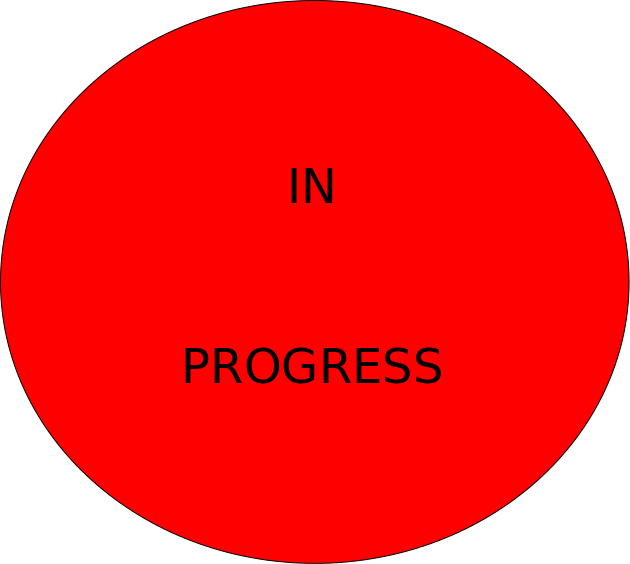
\includegraphics[scale=0.25]{images/in-progress.png}
  \caption[inprogress]{inprogress}
  \label{fig:Bild3.3}
  \end{footnotesize}
\end{figure} 

In the \textit{harmonic/shift} style, the equilibrium distance $r_{0}$ remains constant in time and this is the parameter that must be changed in the LAMMPS code for the swimmer. Modifying and
adding new classes in LAMMPS is not a trivial task as most of them are connected to each other, what can cause problems for compilation or rumble and corrupt results. The new class
\textit{bond harmonic swimmer} was created based on the modification of the \textit{bond harmonic} class. This new  bond style uses the same potential as in \textit{harmonic/shift}, but now $r_{0}$
is not constant anymore and has a sinusoidal variation of the bond length:

\begin{equation}\label{r0}
  r_{0} = A  \sin (\omega x + \phi - Vt)
\end{equation}

where $A$ is the wave amplitude, $\omega$ is the angular frequency, $x$ is the position in x-direction, $\phi$ is the wave phase, $V$ is the wave velocity and $t$ the time.\par
In \textit{bond harmonic/shift} the variable $r_{0}$ is an user input parameter defined in the function \textit{bond$\_$coeff}. In the new bond class, additional user input parameters are 
necessary. The input of $r_{0}$ now is the initial equilibirum distance, where in time this value will added with the sinusoidal function shown in equation~\ref{r0} making $r_{0}$
not constant in time anymore. The new user input parameters are pontential energy $U_{min}$, bond critical distance $r_{c}$, wave amplitude $A$, $\omega$ angular frequency,
the wave phase $\phi$, the wave velocity $V$ and the two particle ID's that forms the bond (the ID's are automatically substracted during the swimmer creation and added in a function
that outputs the \textit{bond$\_$coeff} of all bonds).\par
The \textit{bond harmonic swimmer} bond style will be applied in the  active section of the swimmer tail. When those coefficients are defined in the simulation, it is important to
emphasize that the lower and the upper lines in the active tail have opposite signals in amplitude value. While the upper line bonds are under tension, the lower bonds are under 
compression and vice versa (Figure~\ref{fig:Bild3.4}). With this configuration it is possible to achive a sinusoidal wave thru the whole acitve tail, making the body starts to swim.


\begin{figure}[H]
\centering
  \begin{footnotesize}
  \includesvg{images/bond-mov}
  \caption[Bonds in upper line under tension while bonds in lower line under compression and vice versa]{Bonds in upper line under tension while bonds in lower line under compression and vice versa}
  \label{fig:Bild3.4}
  \end{footnotesize}
\end{figure} 

The code file for the class \textit{bond$\_$harmonic$\_$swimmer} is available in Appendix~\ref{app:bond harmonic swimmer}. 

\section{Bond Style Harmonic Swimmer Extended and Extended K}
\label{sec:section 4}

\subsection{Bond Style Harmonic Swimmer Extended }
\label{sec:section 1}

In chapter 2.2 it is discussed the behaviour of swimmers in nature. When the tail beating pattern of many swimmers , microscopics and macroscopics, was photographically studied
by many authors, it was possible to observe that it is very often that the wave amplitude during swimming it is not contant through the tail. In general, this wave amplitude increases
as it pass through the tail in direction from head to tail tip. One example is the swimming pattern of the snake \textit{Natrix} exhibited in Figure~\ref{fig:Bild2.2}, in the presented set
of photographs it can be seen the amplitude difference near the head and the amplitude in the swimmer tail tip. In \cite{taylor_analysis_1952}, this not constant wave amplitude
pattern in the snake gives a higher swimming efficiency and it reachs higher velocities. Figure~\ref{fig:Bild3.5} shows superposed frames for the snake \textit{Natrix}, it is very
clear to observe this amplitude variation along the tail.\par

\begin{figure}[H]
\centering
  \begin{footnotesize}
  \includesvg{images/snake_swim}
  \caption[]{}
  \label{fig:Bild3.5}
  \end{footnotesize}
\end{figure} 

Based on those studies, it is desired to reproduce this behaviour in our swimmer model created in LAMMPS, and for it is required to create a new bond style to reproduce this swimming
pattern. There are different methods to represent mathematically those changes in the waveform. One method is to represent this wave amplitude change with increasing linearly the 
amplitude value in direction from head to tail, as it is described in \cite{jayne_swimming_1985}. In Equation~\ref{amp} this linear relation for the amplitude value is presented,
where now the wave amplitude depends on which tail segment it is and on the linear equation parameters $a$ and $b$.

\begin{equation}\label{amp}
  A = a X + b
\end{equation}

where $A$ is the amplitude, $X$ is the distance from the head of the swimmer along the direction of travel, and $a$ and $b$ are the linear parameters.\par

A new extended version of the bond style \textit{harmonic/swimmer} must be created to supply the not constant wave amplitude, and the new class is called
\textit{bond$\_$harmonic$\_$swimmer$\_$extended}. In this class, the linear relation is included not only for the ampitude values but also for the angular frequency $\omega$.
The following equation describe how this new approach was included:

\begin{equation}
 r_{0} = A  \sin (\omega x + \phi - Vt)
\end{equation}
 where,
 
\begin{equation}
 A = A_{beta} + dn A_{alpha}
\end{equation}

and
 
\begin{equation}
 \omega = \omega_{beta} + dn \omega_{alpha}
\end{equation}

The parameter $dn$ measures the distance from the tail tip of the swimmer to the head. Due to the parameters already available inside this class, this distance is measured based
on the swimmer particles ID's. The amplitude is now divided in two user input parameters, $A_{alpha}$ and $A_{beta}$ and it is the same for $\omega$, divided in $\omega_{alpha}$
and $\omega_{beta}$.\par


\subsection{Bond Style Harmonic Swimmer Extended K}
\label{sec:section 2}

With the present model described in bond style \textit{harmonic/swimmer/extended}, it is possible to prescribe the swimmer motion with different wave amplitudes, angular frequencies
and velocities. Prescribing the swimmer motion is the most common approach for studies about simulation of swimmers. This approach is sufficient for the kinematics point of view,
but it is not physically consistent.\par
The impulse signals responsible to move the swimmer muscles are sent from the head, propagating along the tail(\cite{jayne_muscular_1988},\cite{gillis_neuromuscular_1998}). This 
impuslse signal decreases its intesity as further it travels along the tail. Considering this concept, it is not phisically logical to have a higher wave amplitude in the tail tip
than in the region near the head. Many other factors can be considered to make this type of motion feasible. In \cite{mchenry_morphology_2005}, it is explained that undulatory 
motion is generated by muscular force and the structural properties of the tail. In many species the tail tip cross section is shorter than the cross section near the head.\par
In Figure~\ref{fig:Bild3.6}, two different larvae, \textit{Herdmania pallida} and \textit{Aplidium constellatum}, have the body shape pictured. It is possible to observe that 
both of them do not have a constant cross section along the tail, and for simulation purposes, it is easier to approximate the real shape by a mean body shape with an elliptical
format. 



\begin{figure}[H]
\centering
  \begin{footnotesize}
  \includesvg{images/cross_sec1}
  \caption[Body shape and tail length of larvae of \textit{Herdmania pallida} and \textit{Aplidium constellatum}\cite{mchenry_morphology_2005}]{Body shape and tail length of larvae of \textit{Herdmania pallida} and \textit{Aplidium constellatum}\cite{mchenry_morphology_2005}}
  \label{fig:Bild3.6}
  \end{footnotesize}
\end{figure} 

Figure~\ref{fig:Bild3.7} is a schematic diagram of a swimming \textit{C. intestinalis} larva with its sensory and motor organs highlighted. The neuromuscular anatomy and its 
transverse section illustrates the anatomy of the tail. With the description of the muscle cells, it becomes easier to visualize the operation of the bonds between tail particles
in the mathematical model. Also, the notochord is represented in our model by the strong internal bonds in the swimmer, as the notochord is stiff in compression and resists shortening,
but it is flexible in bending to allow lateral ondulation. Another interesting point that can be seen from in this picture is the tail  thinning from head to tail tip.


\begin{figure}[H]
\centering
  \begin{footnotesize}
  \includesvg{images/cross_sec2}
  \caption[Schematic diagram of a swimming \textit{C. intestinalis} larva with its sensory and motor organs highlighted]{Schematic diagram of a swimming \textit{C. intestinalis} larva with its sensory and motor organs highlighted}
  \label{fig:Bild3.7}
  \end{footnotesize}
\end{figure} 



Tytell and Hsu \cite{tytell_interactions_2010} introduced the relevance of interactions between internal force, body stiffness and fluid environment. The model presented in this
study includes an actuated, viscoelastic body, based on that of a lamprey swimming. The motion of the body emerges as a balance between internal muscular force and eternal fluid
forces. Depending on external parameters such as viscosity and internal parameters such as body stiffness, the swimmer can achieve different levels of performance, including
rapid acceleration or high speed. In this same study, the axial impulse per unit height produced during steady swimming is studied. It is seen that the impulse value increases with the position
along the body of the swimming lamprey. This dependency of body stiffiness in swimming performance was studied by Tytell and Hsu and it is shown in Figure~\ref{fig:Bild3.8}
\par


\begin{figure}[H]
\centering
  \begin{footnotesize}
  \includesvg{images/body_stiff}
  \caption[For a given muscle activation pattern, there are different optimal stiffness values for maximum acceleration or steady swimming speed.The plots show four swimmers 
  with increasing stiffness: tan dotted line, simulation 4, Table 1; green long dashes, simulation 5; black, reference simulation; and cyan short dashes, simulation 6. (A)
  Swimming speed vs. time. (B)Body outlines for each swimmer at the time indicated by the arrow on panel. (C) Mean acceleration during the first tail beat. (D) Mean steady
  swimming speed. (E) Muscle power coefficient]{For a given muscle activation pattern, there are different optimal stiffness values for maximum acceleration or steady swimming speed.The plots show four swimmers 
  with increasing stiffness: tan dotted line, simulation 4, Table 1; green long dashes, simulation 5; black, reference simulation; and cyan short dashes, simulation 6. (A)
  Swimming speed vs. time. (B)Body outlines for each swimmer at the time indicated by the arrow on panel. (C) Mean acceleration during the first tail beat. (D) Mean steady
  swimming speed. (E) Muscle power coefficient. \cite{tytell_interactions_2010}}
  \label{fig:Bild3.8}
  \end{footnotesize}
\end{figure} 






After assembling all information presented here about the swimmer motion and physiology, a new mathematical model was created to combine all requirements to get closer to a more
realistic model than the regular prescribed motion model. In this model, instead of creating some mathematical relation to increase amplitude along the swimmer body based on the
amplitude value, the body stiffness is decreased along the body from head to tail. This  approach goes in a realistic direction as many swimmers , as larvae of \textit{Herdmania pallida} and
\textit{Aplidium constellatum}, has a cross section thinning along the body, and this behaviour can be approached reducing the body stiffness along the body. This new model was
implemented in LAMMPS and the results are shown in Chapter 4. \par

In LAMMPS, a new class was created, called \textit{bond$\_$harmonic$\_$swimmer$\_$extended$\_$k}, to describe this bond style. In this bond style, the wave parameters remained the same, i.e. all previous configurations can be also set with this new class. 
Previously, the bond stiffness inside the class was defined as:

\begin{equation}
 K = \frac{U_{min}}{( r_{0} - r_{c})^2} ,
\end{equation}

and now a linear relation was added to this new class, that means that the bond stiffness will linear decrease along the body. This relation is set as:

\begin{equation}
 K = K_{beta} + dn K_{alpha}
\end{equation}

and

\begin{equation}
 K_{alpha} = \frac{U_{min}}{( r_{0} - r_{c})^2} ,
\end{equation}


where $K_{alpha}$ and $K_{beta}$ are the linear parameters to give the local stiffness value and $dn$ measures the distance from the tail tip of the swimmer to the head, as before
in previous bond style.\par

The user input parameters are the same as before except for the addition of $K_{beta}$. The parameter $K_{alpha}$ is inside calculated based on the potential energy user
input $U_{min}$. In Appendix~\ref{app:bond harmonic swimmer ext k}, the code file for the \textit{bond$\_$harmonic$\_$swimmer$\_$extended$\_$k} is presented, which include also
the modification done in \textit{bond$\_$harmonic$\_$swimmer$\_$extended}.








\section{SPH Kernel Class}
\label{sec:section 5}

The main point of smooth particle hydronamics lie on the kernel interpolants. In particular, a kernel summation interpolant is used for estimating the density
which then govern the rest of the basic SPH equations through the variational formalism. The performance of a SPH model depends on the choice of the wiegthing functions. \par
For any field $F(r)$, a smoothed interpolated version can be defined, $F_{s}(r)$, through a convolution with a kernel $W(r,h)$:

\begin{equation}
 F_{s}(r) = \int F(r') W(r-r',h)dr' ,
\end{equation}

where $h$ describes width of the kernel (smoothing length), which is normalised to unity and approximates a Dirac $\delta$-function in the limit $h\rightarrow 0$. This kernel must be symmetric
and sufficiently smooth to make it at least differentiable twice. Figure~\ref{fig:Bild3.9} is a sketch of the influence domain decribed by the smoothing length $h_{i}$ and the influenced
point $i$


\begin{figure}[H]
\centering
  \begin{footnotesize}
  \includesvg{images/kernel}
  \caption[Sketch of the smoothing kernel length $h_{i}$ and its influence domainSketch of the smoothing kernel length $h_{i}$ and its influence domain]{Sketch of the smoothing kernel length $h_{i}$ and its influence domain}
  \label{fig:Bild3.9}
  \end{footnotesize}
\end{figure} 

There are some important properties that the smoothing function must fulfill. It must be normmalised:

\begin{equation}
 \int_{\Omega}W(r-r',h)dr'= 1 ,
\end{equation}

it should be compactly supported , should be monotonically decreasing with the distance awy from the particle and also, should satisfy the Dirac delta function condition as the smoothing
length approaches to zero 

\begin{equation}
 \lim_{h\to 0} W(r-r',h)= \delta(r-r') ,
\end{equation}

There are many different methods to describe the weighting function $W$. Monaghan and Gingold \cite{gingold_smoothed_1977} introduced first a Gaussian kernel. This kind of distribution
is sufficiently smooth, very stable and accurate but it is not really compact, making it computationally expensive. Equation~\ref{gauss} is a Gaussian distribution for the kernel
and Figure~\ref{fig:Bild3.10} a Gaussian kernel is plotted and an illustrative picture shows how in the Gaussian distribution set in a particle domain.

\begin{equation}\label{gauss}
 W(r-r',h) = \frac{\sigma}{h^d} exp[-\frac{(r-r')^2}{h^2}] ,
\end{equation}

where $d$ refers to the number of spatial dimensions is a normalisation factor given in 3 dimensions given by:

\begin{equation}
 \sigma = [1/\sqrt{\pi},1/\pi,1/(\pi\sqrt{\pi})]
\end{equation}

\begin{figure}[H]
\centering
  \begin{footnotesize}
  \includesvg{images/gauss}
  \caption[Gaussian kernel plotted with $R=\frac{|r-r'|}{h}$ and Gaussian distribution in particle domain]{Gaussian kernel plotted with $R=\frac{|r-r'|}{h}$ and Gaussian distribution in particle domain}
  \label{fig:Bild3.10}
  \end{footnotesize}
\end{figure} 

Another smoothing function used is the cubic spline or B-spline, which is the most popular used in SPH (\cite{monaghan_refined_1985}). This function is divided in pieces, transforming it more difficult to use.
This gives a progresively better approximations to the Gaussian at higher number of particles by increasing the radius of compact support and by increasing smoothness. Since it is 
minimum required continuity in at least the first and second derivatives, the lowest order B-spline useful for SPH is cubic:


\begin{equation}
 w(q) = \sigma \left\{
  \begin{array}{l l}
 \frac{1}{4} (2-q)^3 - (1-q)^3, & 0\le q < 1 ;\\
 \frac{1}{4} (2-q)^3, &  1\le q < 2 ;\\
 0. & q\ge 2,
  \end {array}\right.\
\end{equation}


where for convenience $W(|r-r'|,h)\equiv \frac{1}{h^d} w(q)$, $q = |r-r'/h|$ and here, $\sigma$ is given by $\sigma = [2/3,10/(7\pi),1/\pi]$ in $[1,2,3]$ dimensions.Figure~\ref{fig:Bild3.11}
shows a plot for B-spline functions comparedto Gaussian functions.

\begin{figure}[H]
\centering
  \begin{footnotesize}
  \includesvg{images/cubic}
  \caption[B-spline function plotted compared to Gaussian distribution]{B-spline function plotted compared to Gaussian distribution}
  \label{fig:Bild3.11}
  \end{footnotesize}
\end{figure} 

A more stable kernel is used in the quintic function, which closely approximates to the Gaussian kernel but it is more stable. For the quintic function, the normalisation is
$\sigma = [1/24,96/(1199\pi),1/20\pi]$ and its weighting function is written below. Figure~\ref{fig:Bild3.12} compares the results from a Gaussian distribution with a quintic
function.

 \begin{equation}
 w(q) = \sigma \left\{
  \begin{array}{l l}
 (3-q)^5 - 6(2-q)^5 + 15(1-q)^5, & 0\le q < 1 ;\\
 (3-q)^5- 6(2-q)^5, &  1\le q < 2 ;\\
 (3-q)^5, &  2\le q < 3;\\
 0. & q\ge 3,
  \end {array}\right.\
\end{equation}


\begin{figure}[H]
\centering
  \begin{footnotesize}
  \includesvg{images/quintic}
  \caption[Quintic function plotted compared to Gaussian distribution]{Quintic function plotted compared to Gaussian distribution}
  \label{fig:Bild3.12}
  \end{footnotesize}
\end{figure} 



LAMMPS proposes only one type of kernel, a Lucy kernel \cite{lucy_numerical_1977}. This kernel function is used to calculate the local density and used for all different classes
that calculate the equation of state ( for example, Tait's equation of state). The form of Lucy kernel function is shown below:


\begin{equation}
 W(r<h) = \frac{1}{s}\left[1 +3 \frac{r}{h}\right]\left[1-\frac{r}{h}\right]^3 ,
\end{equation}
 
Here, $s$ is the normalisation factor which depends on the number of spatial dimensions, in LAMMPS implmented for 2D and 3D. \par

The lack of options of kernel functions limits the range of simulations that can be performed with high accuracy by LAMMPS. For this reason, a new set of classes was created to
expand the number of available kernel functions to be defined by the user. Initially the kernel functions are included into the classes where it is requested, as calculating local 
density in \textit{pair$\_$style sph/rhosum}, in \textit{pair$\_$style sph/taitwater}, in Lennard-Jones equation of state \textit{pair$\_$style sph/lj} and all others SPH
\textit{pair$\_$style}. \par

A base class to include new kernel functions was created as \textit{sph$\_$kernel}. Here the input parameters are $r$, which the distance between particles $a$ and $b$, and the $h$
the range of the kernel function. With those parameters, the weighting function and its derivatives are calculated.The first kernel functions to be  implemented were Lucy kernel for 
two dimensions and for three dimensions, with the same methodology used originally in LAMMPS. The next kernel function added was a quadratic function described bellow:

\begin{equation} 
 W(r<h) = 1.5915(r-h)^4\frac{(r+h)^4}{h^{10}} ,
\end{equation}
 
and its derivative

\begin{equation}
 dW(r<h) = 12.7323r(r-h)^3\frac{(r+h)^3}{h^{10}}
\end{equation}
 
This particular form of the quadratic kernel function is diretcly implemented in the new class and for a two-dimensional case. In LAMMPS, this new class was called
\textit{sph$\_$kernel$\_$quadric$\_$2d} and another class for a three-dimensional case was also created.\par

The last kernel function included in LAMMPS the quintic kernel. The weighting functions used is described bellow:


  \begin{equation}
 w(s) = \sigma \left\{
  \begin{array}{l l}
 (3-s)^5 - 6(2-s)^5 + 15(1-s)^5, & 0\le s < 1 ;\\
 (3-s)^5- 6(2-s)^5, &  1\le s < 2 ;\\
 (3-s)^5, &  2\le s < 3;\\
 0. & s\ge 3,
  \end {array}\right.\
\end{equation}

where

\begin{equation}
 \sigma = \frac{0.04195}{h^2} \text{,for 2D} \quad \text{and} \quad \sigma = \frac{0.12585}{h^3} \text{,for 3D}
\end{equation}

and 

\begin{equation}
 s = \frac{3r}{h}
\end{equation}

A new user input coefficient is included for all SPH \textit{pair styles}, which is the kernel function type: lucy, quadric or quintic. One example of the kernel function classes
that were add in LAMMPS is available in Appendix~\ref{app:kernel function}.









